
% This LaTeX was auto-generated from MATLAB code.
% To make changes, update the MATLAB code and republish this document.











    
    \begin{DoxyCode}
clear
\end{DoxyCode}
\begin{par}
COMPILATION
\end{par} \vspace{1em}
\begin{DoxyCode}
[exdir,~,~]=fileparts(which('example_model_3.m'));
% compile the model
amiwrap('model_example_3','example_model_3_syms',exdir)
% add the model to the path
addpath(genpath([strrep(which('amiwrap.m'),'amiwrap.m','') 'models/model_example_3']))
\end{DoxyCode}

         \begin{DoxyCode}Generating model struct ...
Parsing model struct ...
Generating C code ...
headers | wrapfunctions | 
Compiling mex file ...
Building with 'Xcode with Clang'.
MEX completed successfully.
\end{DoxyCode} 
    \begin{par}
SIMULATION
\end{par} \vspace{1em}
\begin{DoxyCode}
% time vector
t = linspace(0,300,20);
p = [1;0.5;0.4;2;0.1];
k = [0.1,0.4,0.7,1];

options.sensi = 0;
options.cvode_maxsteps = 1e6;
% load mex into memory
sol = simulate_model_example_3(t,log10(p),k,[],options);

tic
sol = simulate_model_example_3(t,log10(p),k,[],options);
disp(['Time elapsed with cvodes: ' num2str(toc) ])
\end{DoxyCode}

         \begin{DoxyCode}Time elapsed with cvodes: 0.002146
\end{DoxyCode} 
    \begin{par}
ODE15S
\end{par} \vspace{1em}
\begin{DoxyCode}
ode_system = @(t,x,p,k) [-2*p(1)*x(1)^2 - p(2)*x(1)*x(2) + 2*p(3)*x(2) + p(4)*x(3) + p(5);
    + p(1)*x(1)^2 - p(2)*x(1)*x(2) - p(3)*x(2) + p(4)*x(3);
    + p(2)*x(1)*x(2) - p(4)*x(3) - k(4)*x(3)];
options_ode15s = odeset('RelTol',1e-8,'AbsTol',1e-8,'MaxStep',1e4);

tic
[~, X_ode15s] = ode15s(@(t,x) ode_system(t,x,p,k),t,k(1:3),options_ode15s);
disp(['Time elapsed with ode15s: ' num2str(toc) ])
\end{DoxyCode}

         \begin{DoxyCode}Time elapsed with ode15s: 0.18018
\end{DoxyCode} 
    \begin{par}
PLOTTING
\end{par} \vspace{1em}
\begin{DoxyCode}
figure
c_x = get(gca,'ColorOrder');
subplot(2,2,1)
for ix = 1:size(sol.x,2)
    plot(t,sol.x(:,ix),'.-','Color',c_x(ix,:))
    hold on
    plot(t,X_ode15s(:,ix),'d','Color',c_x(ix,:))
end
legend('x1','x1_{ode15s}','x2','x2_{ode15s}','x3','x3_{ode15s}','Location','NorthEastOutside')
legend boxoff
xlabel('time t')
ylabel('x')
box on
subplot(2,2,2)
plot(t,abs(sol.x-X_ode15s),'--')
set(gca,'YScale','log')
legend('error x1','error x2','error x3','Location','NorthEastOutside')
legend boxoff
set(gcf,'Position',[100 300 1200 500])
\end{DoxyCode}

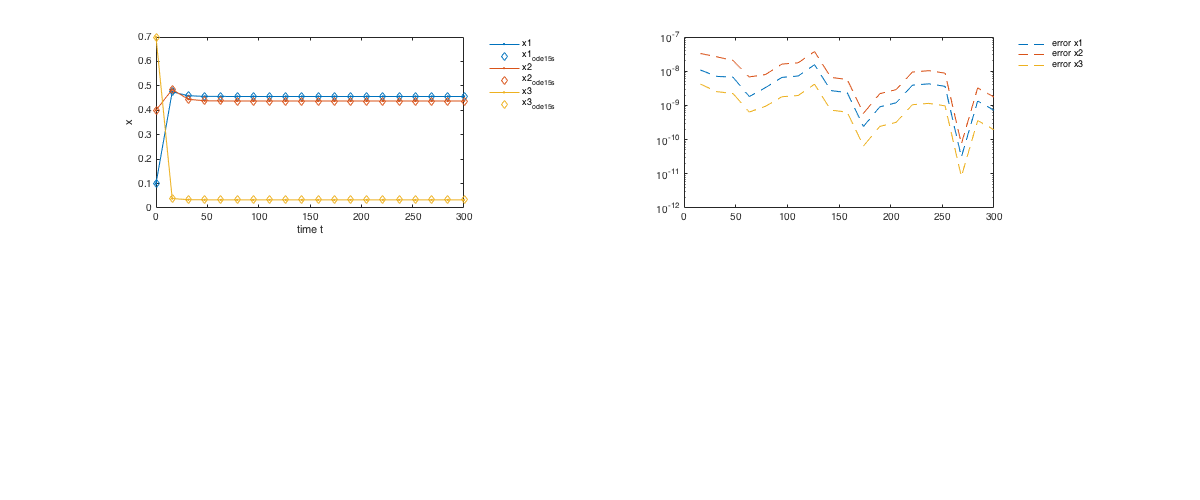
\includegraphics [width=4in]{../../examples/example_3/html/example_model_3_01.png}
\begin{par}
FORWARD SENSITIVITY ANALYSIS
\end{par} \vspace{1em}
\begin{DoxyCode}
options.sensi = 1;
options.sens_ind = [3,1,2,4];

sol = simulate_model_example_3(t,log10(p),k,[],options);
\end{DoxyCode}
\begin{par}
FINITE DIFFERENCES
\end{par} \vspace{1em}
\begin{DoxyCode}
eps = 1e-3;

xi = log10(p);
for ip = 1:4;
    xip = xi;
    xip(ip) = xip(ip) + eps;
    solp = simulate_model_example_3(t,xip,k,[],options);
    sx_fd(:,:,ip) = (solp.x - sol.x)/eps;
    sy_fd(:,:,ip) = (solp.y - sol.y)/eps;
end
\end{DoxyCode}
\begin{par}
PLOTTING
\end{par} \vspace{1em}
\begin{DoxyCode}
figure
for ip = 1:4
    subplot(4,2,ip*2-1)
    hold on
    for ix = 1:size(sol.x,2)
        plot(t,sol.sx(:,ix,ip),'.-','Color',c_x(ix,:))
        plot(t,sx_fd(:,ix,options.sens_ind(ip)),'d','Color',c_x(ix,:))
    end
    legend('x1','x1_{fd}','x2','x2_{fd}','x3','x3_{fd}','Location','NorthEastOutside')
    legend boxoff
    title(['state sensitivity for p' num2str(options.sens_ind(ip))])
    xlabel('time t')
    ylabel('x')
    box on

    subplot(4,2,ip*2)
    plot(t,abs(sol.sx(:,:,ip)-sx_fd(:,:,options.sens_ind(ip))),'--')
    legend('error x1','error x2','error x3','Location','NorthEastOutside')
    legend boxoff
    title(['error of state sensitivity for p' num2str(options.sens_ind(ip))])
    xlabel('time t')
    ylabel('error')
    set(gca,'YScale','log')
    box on
end
set(gcf,'Position',[100 300 1200 500])
\end{DoxyCode}

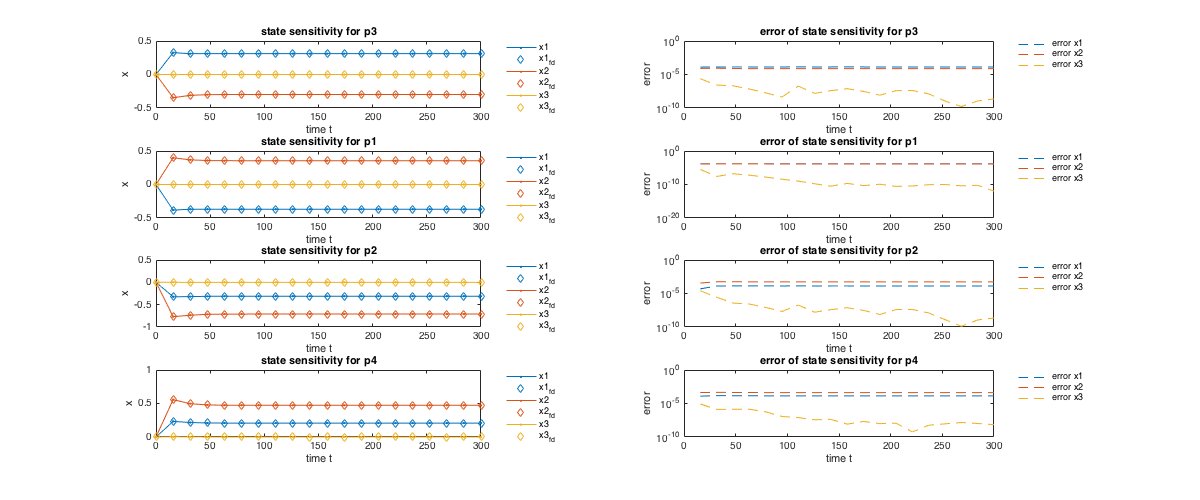
\includegraphics [width=4in]{../../examples/example_3/html/example_model_3_02.png}
\begin{par}
STEADY STATE SENSITIVITY
\end{par} \vspace{1em}
\begin{DoxyCode}
sssens = NaN(size(sol.sx));
for it = 2:length(t)
    tt = [0,t(it)];
    options.sensi_meth = 'ss';
    solss = simulate_model_example_3(tt,log10(p),k,[],options);
    sssens(it,:,:) = solss.sx;
    ssxdot(it,:) = solss.xdot;
end
\end{DoxyCode}
\begin{par}
PLOTTING
\end{par} \vspace{1em}
\begin{DoxyCode}
figure
for ip = 1:4
    subplot(4,2,ip*2-1)
    hold on
    for ix = 1:size(sol.x,2)
        plot(t,sol.sx(:,ix,ip),'.-','Color',c_x(ix,:))
        plot(t,sssens(:,ix,ip),'d-','Color',c_x(ix,:))
    end
    legend('x1','x1_{ss}','x2','x2_{ss}','x3','x3_{ss}','Location','NorthEastOutside')
    legend boxoff
    title(['state steady sensitivity for p' num2str(ip)])
    xlabel('time t')
    ylabel('x')
    box on

    subplot(4,2,ip*2)
    plot(t,abs(sol.sx(:,:,ip)-sssens(:,:,ip)),'--')
    legend('error x1','error x2','error x3','Location','NorthEastOutside')
    legend boxoff
    title(['error of steady state sensitivity for p' num2str(ip)])
    xlabel('time t')
    ylabel('error')
    set(gca,'YScale','log')
    box on
end
set(gcf,'Position',[100 300 1200 500])

figure
scatter(sqrt(sum((ssxdot./sol.x).^2,2)),sqrt(sum(sum((sol.sx-sssens).^2,2),3)))
hold on
plot([1e-15,1e5],[1e-15,1e5],'k:')
set(gca,'YScale','log')
set(gca,'XScale','log')
box on
axis square
xlabel('||dxdt/x||_2')
ylabel('error steady state approximation')
set(gca,'FontSize',15)
set(gca,'LineWidth',1.5)
set(gcf,'Position',[100 300 1200 500])
\end{DoxyCode}

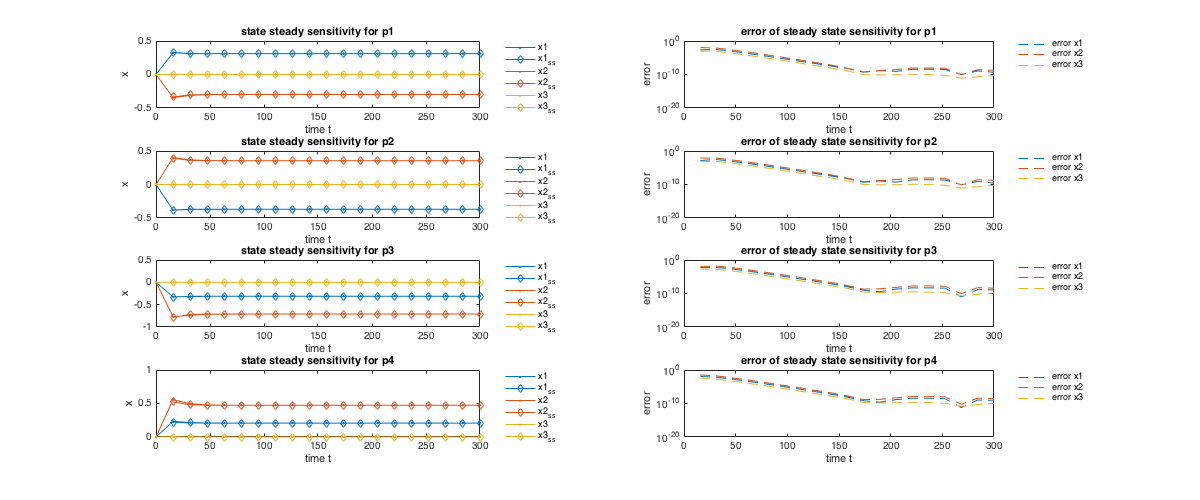
\includegraphics [width=4in]{../../examples/example_3/html/example_model_3_03.png}

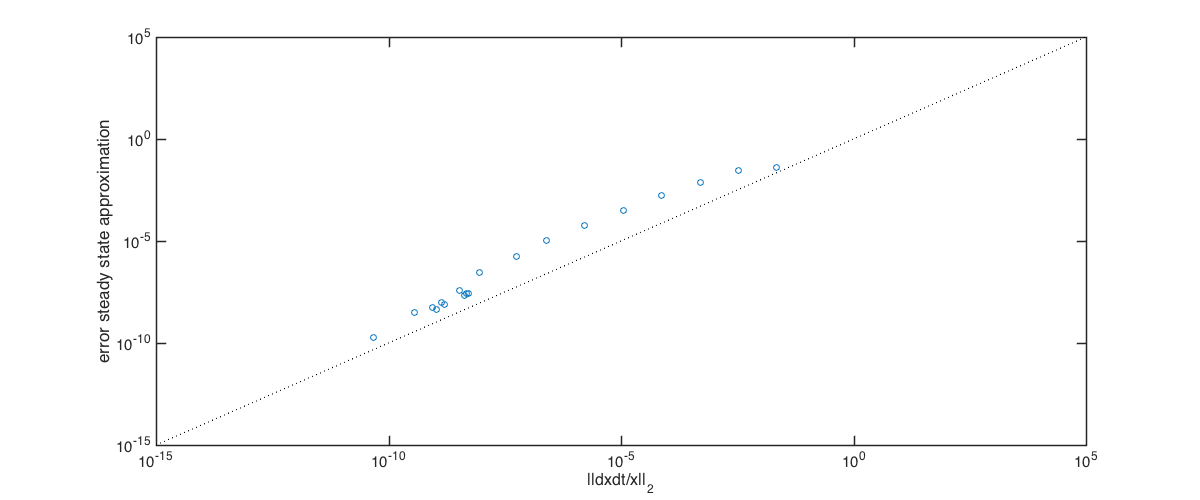
\includegraphics [width=4in]{../../examples/example_3/html/example_model_3_04.png}




    